This section aims to show more in detail the calculation procedure. The methodology is applied to a basic power system such as the 5-bus system from the GridCal tutorial \cite{gridcal}, shown in Fig. \ref{fig:5bus}. 

\begin{figure}[!htb]\centering
  \begin{tikzpicture}
    \draw (0,0) to [sinusoidal voltage source] (-0.6,0.6);
    \draw (-0.6,0.6) to [short] (-1,1);
    \draw (-1,1) to [short] (-1,1.2);
    \draw[ultra thick] (-0.8,1.2) to [short] (-1.6,1.2);
    \draw (-1.4,1.2) to [short] (-1.4,1.0);
    \draw (-1.4,1.0) to [short] (-2.9,-0.5);
    \draw (-2.9,-0.5) to [short] (-2.9,-0.7);
    \draw (-3.3,-0.7) to [short] (-3.3,3.1);
    \draw (0.9,-0.7) to [short] (0.9,3.1);

    \draw (-2.9,3.1) to [short] (-2.9,3.3);
    \draw (-2.9,3.3) to [short] (0.5,3.3);
    \draw (0.5,3.3) to [short] (0.5,3.1);

    \draw (-2.9,-0.7) to [short] (-2.9,-0.9);
    \draw (-2.9,-0.9) to [short] (0.5,-0.9);
    \draw (0.5,-0.9) to [short] (0.5,-0.7);

    \draw (-1.0,1.2) to [short] (-1,1.4);
    \draw (-1.0,1.4) to [short] (0.5,2.9);
    \draw (0.5,2.9) to [short] (0.5,3.1);
    \draw (-1.4,1.2) to [short] (-1.4,1.4);
    \draw (-1.4,1.4) to [short] (-2.9,2.9);
    \draw (-2.9,2.9) to [short] (-2.9,3.1);

    \draw[ultra thick] (-2.7,-0.7) to [short] (-3.5, -0.7);
    \draw[ultra thick] (-2.7,3.1) to [short] (-3.5,3.1);
    \draw[ultra thick] (0.3,3.1) to [short] (1.1,3.1);
    \draw[ultra thick] (0.3,-0.7) to [short] (1.1,-0.7);

    \draw[-{Latex[scale=1.5]}] (-3.3,-0.7) -- (-3.3,-1.5);
    \draw[-{Latex[scale=1.5]}] (0.9,-0.7) -- (0.9,-1.5);
    \draw[-{Latex[scale=1.5]}] (-3.3,3.1) -- (-3.3,3.9);
    \draw[-{Latex[scale=1.5]}] (0.9,3.1) -- (0.9,3.9);

    \node(bus5) at (-3.7,-0.7) {5};
    \node(bus2) at (-3.7,3.1) {2};
    \node(bus3) at (1.3,3.1) {3};
    \node(bus4) at (1.3,-0.7) {4};
    \node(bus1) at (-0.6,1.2) {1};
  \end{tikzpicture}
  \caption{High-level representation of the 5-bus system}
  \label{fig:5bus}
\end{figure}
The system is formed by four PQ buses and one slack bus, corresponding to node 1. Lines are originally modeled with a $\pi$ equivalent. Nevertheless, the parallel capacitances are removed to have voltages below the level imposed by the slack bus, which should help in obtaining a more intuitive result. 

The state of interest will be the voltage magniude at bus 5, thus, $x=V_5$. Chosing the parameters is rather a subjective choice which largely depends on the scope of the study. However, they are chosen to be the four active powers and the four reactive powers in this case:
\begin{equation}
  [p_1,p_2,p_3,p_4,p_5,p_6,p_7,p_8] = [P_2,Q_2,P_3,Q_3,P_4,Q_4,P_5,Q_5],
  \label{eq:params}
\end{equation}
where $P$ and $Q$ stand for the loads of active and reactive power. 

These powers can take any value inside a predefined range of values. In a realistic scenario, this range could comprise a high confidence interval. Table \ref{tab:lowup} shows the chosen lower and upper bounds for all powers.  

\begin{table}[!htb]
  \centering
  \begin{tabular}{lcccccccc}
    \hline
    Limit & $P_2$ & $Q_2$ & $P_3$ & $Q_3$ & $P_4$ & $Q_4$ & $P_5$ & $Q_5$ \\
    \hline
    Lower & 0 & 0 & 0 & 0 & 0 & 0 & 0 & 0 \\
    Upper & 40 & 30 & 30 & 45 & 25 & 20 & 30 & 20 \\
    \hline
  \end{tabular}
  \caption{Lower and upper limit for all parameters, in the order of MVA}
  \label{tab:lowup}
\end{table}
The calculation process obeys the four steps summarized in Section \ref{sec:process}. Each of them is numerically detailed below. 

\hspace{0.32cm} 1. Compute the gradients for the $M$ samples to calculate the covariance matrix $\mathbf{C}$ with \eqref{eq:C1}. 

A total of $M=10$ samples is chosen. This becomes a reasonable amount considering that the expansion order is set to $l=3$. Moreover, as it will be shown in the next step, all eight parameters will be encapsulated in a single meaningful direction, so $k=1$. Thus, $N_t = 4$ in accordance with \eqref{eq:Nt1}. The requirements are being met since $M$ should be between 1.5 to 3 times $N_t$.

There is no complexity in genereting the samples. All parameters take random values between the limits set in Table \ref{tab:lowup}. The power flow is solved $M(m+1) = 10(8 + 1)=90$ times. With it, a total of 10 gradients are obtained by following \eqref{eq:grad2}. The covariance matrix $\mathbf{C}$ is built by adding the products of gradients, as shown in \eqref{eq:C1}. In this particular case, it becomes:
\begin{equation}
  \mathbf{C} = 10^{-8} \cdot \begin{pmatrix}
 1.39 & 3.18 &  1.93 & 4.40 & 5.00 &  11.16 & 1.92 & 4.57 \\
 3.18 & 7.27 &  4.40 &  10.05 & 11.41 &25.48 & 4.39 & 10.43 \\
 1.93 & 4.40 &   2.66 & 6.08 & 6.91 &  15.43 & 2.66 & 6.31 \\
 4.40 & 10.05 & 6.08 & 13.89 & 15.77 &  35.21 & 6.07 & 14.41 \\
 5.00 & 11.41 & 6.91 & 15.77 & 17.91 & 39.98 & 6.89 &  16.36 \\ 
 11.16 &25.48 & 15.43 &35.21 &39.98 & 89.28 &  15.39 &36.54 \\
 1.92 & 4.39 &  2.66 & 6.07 & 6.89 &   15.39 & 2.65 & 6.30 \\
 4.57 &  10.43 & 6.31 & 14.41 & 16.36 & 36.54 & 6.30 & 14.95 \\
  \end{pmatrix}.
  \label{eq:Cres}
\end{equation}
It is symmetrical, with tiny values as the voltage does not change much with variations in the powers.

\hspace{0.32cm} 2. Perform the orthogonal decomposition of $\mathbf{C}$ and select the most influential dimensions according to the desired truncation error. 

The orthogonal decomposition of the covariance matrix follows \eqref{eq:C2}. The eight eigenvalues are presented in Table \ref{tab:eigenv}. 

\begin{table}[!htb]
  \centering
  \begin{tabular}{lcccccccc}
    \hline
     & $\lambda_1$ & $\lambda_2$ & $\lambda_3$ & $\lambda_4$ & $\lambda_5$ & $\lambda_6$ & $\lambda_7$ & $\lambda_8$ \\
    \hline
    Value ($\cdot 10^{-12}$) & 1.5$\cdot 10^{6}$ & 67 & 28 & 21 & 5 & 3 & 1 & 0 \\
    \hline
  \end{tabular}
  \caption{Ordered eigenvalues obtained from the orthogonal decomposition}
  \label{tab:eigenv}
\end{table}
The first eigenvalue is significantly more relevant than the others. Choosing $k=1$ impactful dimensions translates into a minuscule truncation error. This shows that going from 8 to 1 dimension is possible without making a notorious mistake. 

As $k=1$, $\mathbf{W}_y$ is a single-column matrix containing the eigenvector $\mathbf{w}_1$ associated with $\lambda_1$:
\begin{equation}
  \mathbf{W}_y = \begin{pmatrix}
 0.096509323157 \\
 0.220170675384 \\
 0.133325972120 \\
 0.304257354543 \\
 0.345498102071 \\
 0.771423934788 \\
 0.133032385496 \\
 0.315754699603 \\
  \end{pmatrix}.
  \label{eq:eigenvec}
\end{equation}
This matrix weights all parameters. Notice how the sixth parameter, the one corresponding to $P_4$, is the largest by far. This could also have been observed in the $\mathbf{C}$ matrix shown in \eqref{eq:Cres}, where the sixth column/row has significantly greater values than the rest. It makes sense that $P_4$ has a notable impact on $V_5$ because bus 4 is the only one not directly connected to the slack bus. 

\hspace{0.32cm} 3. With the random samples, transform $\mathbf{p}$ into $\mathbf{y}$ with \eqref{eq:y1}. 

Then, the $\mathbf{p}$ vector with the random samples and the matrix $\mathbf{W}_y^T$ are multiplied for all samples. This is a straightforward step since the two involved objects are already known. The goal is to transform the 8 dimensions in $\mathbf{p}$ to just one dimension stored in $\mathbf{y}$. In the end, the procedure looks for $h(\mathbf{y})$, so $\mathbf{p}$ always has to be transformed. 

Since there is only one dimension in $\mathbf{y}$, the basis function expansion turns out to be simplified. If $l=3$:
\begin{equation}
  h(y) = c_0 + c_1 \cdot y^1 + c_2 \cdot y^2 + c_3 \cdot y^3,
  \label{eq:hy}
\end{equation}
where $y \in \mathbb{R}$ and the coefficients $c$ have to be calculated.  

\hspace{0.32cm} 4. Build the $\mathbf{Q}$ matrix, the $\mathbf{h_x}$ vector, and find the coefficients with \eqref{eq:lss2}. 

The $\mathbf{h_x}$ vector has been previously computed. It simply gathers the 10 solutions (one for each sample) of $V_5$, and is equal to:
\begin{equation}
  \mathbf{h_x} = \begin{pmatrix}
0.95989933482 \\
0.956904257759 \\
0.956758440075 \\
0.964702869164 \\
0.957956346033 \\
0.965846162026 \\
0.973066025427 \\
0.961498057762 \\
0.956583704834 \\
0.966603851952 \\
  \end{pmatrix}.
  \label{eq:vech}
\end{equation}
The $\mathbf{Q}$ matrix has dimensions $10 \times 4$, and it is formed by the four elements that are multiplied by the coefficients in \eqref{eq:hy}, with each sample constituting a row. It is not shown here for simplicity. 

Finally, the coefficients in $\mathbf{c}$ are computed with \eqref{eq:lss2}. The resulting equation becomes:
\begin{equation}
  \boxed{
    \begin{split}
      V_5 \approx h(y) = 1.000044024546 -1.147157669\cdot 10^{-3} y & -1.101177\cdot 10^{-6} y^2 \\ & -3.244\cdot 10^{-9} y^3.
\end{split}
}
  \label{eq:final}
\end{equation}
To calculate the approximated voltage in every possible situation it is enough to convert the vector of parameters $\mathbf{p}$ to $y$ and input its value to \eqref{eq:final}. Fig. \ref{fig:V5y} shows the value $V_5$ takes depending on $y$. 

\begin{figure}[!htb] \centering
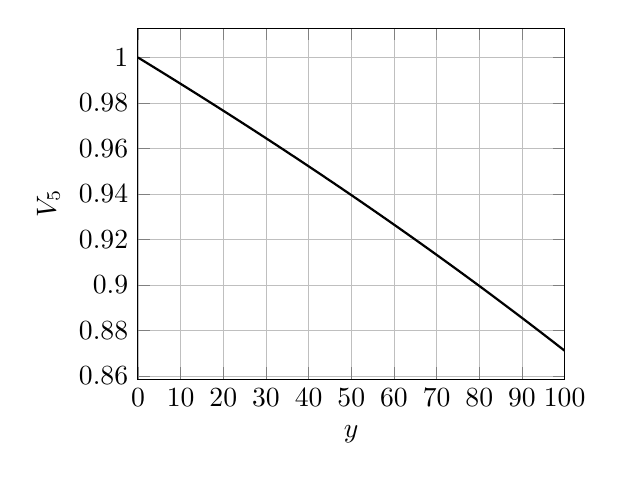
\begin{tikzpicture}
  \begin{axis}[xlabel={$y$}, ylabel={$V_5$}, grid=both, grid style={line width=.1pt, draw=gray!10}, major grid style={line width=.2pt,draw=gray!50}, xtick distance = 10, ytick distance = 0.02, width=7cm, every plot/.append style={very thick}, xmin = 0, xmax = 100]
\addplot [
    style=thick,
    domain=0:100,
    samples = 400] 
    % {1 + 0.1 * x};
    {1.000044024546 - 0.001147157669 * x - 0.000001101177 * x^2 - 0.000000003244 * x^3};
\end{axis}
\end{tikzpicture}
\caption{Graphical interpretation of $V_5 \approx h(y)$}
\label{fig:V5y}
\end{figure}
If the horizontal axis were to be extended, it would become clear how $V_5(y)$ follows a parabolic profile, similar to the typical P-V curves. Also, it is relevant to mention that the values of $\mathbf{h_x}$ are around 0.95 to 0.98 approximately. This is due to the lower and upper bounds defined in \ref{tab:lowup}. Therefore, the computed value of $y$ should be between 15 and 40 more or less.

The methodology has been tested for several cases with satisfactory results. Table \ref{tab:res} compares the results obtained with $V_5 \approx h(y)$ and the results provided by the power flow solver in case $\mathbf{p} = [25, 12, 8, 33, 21, 4, 17, 11]$ MVA. 

\begin{table}[!htb]\centering
  \begin{tabular}{lc}
  \hline
  Magnitude & Value \\
  \hline
  $V_5$ from \eqref{eq:final} & 0.9618089693761898\\
  $V_5$ from the power flow solver & 0.9618607699599497\\
  Error & 5.180058375997554$\cdot 10^{-5}$\\
  \hline
\end{tabular}
  \caption{Comparison of results when $\mathbf{p} = [25, 12, 8, 33, 21, 4, 17, 11]$ MVA}
  \label{tab:res}
\end{table}
It can be concluded that by only calling the power flow 90 times, a satisfactory model has been obtained. It can reproduce with great accuracy the actual $V_5$ value as a function of the parameters. 

In essence, the methodology is based on computing the gradients at different operating points. It may seem equally valid to calculate the gradient at a random operating point and estimate the state from this. While this basic approach could work for grids where the loads are at their lower levels, it is not suitable for higher load levels. Intuitively speaking, the operating points would move closer to the nose of the P-V curves, which are quadratic. As a consequence, a simple linearization at a random point becomes sub-optimal. 



% put a box around the final equation with y!!

